

\documentclass{article}

\usepackage[version=3]{mhchem} % Package for chemical equation typesetting
\usepackage{siunitx} % Provides the \SI{}{} and \si{} command for typesetting SI units
\usepackage{graphicx} % Required for the inclusion of images
\usepackage{natbib} % Required to change bibliography style to APA
\usepackage{amsmath} % Required for some math elements 
\usepackage[margin=1.2in]{geometry}
\setlength\parindent{0pt} % Removes all indentation from paragraphs

\renewcommand{\labelenumi}{\alph{enumi}.} % Make numbering in the enumerate environment by letter rather than number (e.g. section 6)

%\usepackage{times} % Uncomment to use the Times New Roman font

%----------------------------------------------------------------------------------------
%	DOCUMENT INFORMATION
%----------------------------------------------------------------------------------------

\title{11-741 k-means Clustering} % Title

\author{Xin Qian, xinq} % Author name

\date{\today} % Date for the report

\begin{document}

\maketitle % Insert the title, author and date

\begin{center}
\begin{tabular}{l r}
Due: Sept 22, 2016 11:59 PM\end{tabular}
\end{center}

% If you wish to include an abstract, uncomment the lines below
% \begin{abstract}
% Abstract text
% \end{abstract}

%----------------------------------------------------------------------------------------
%	SECTION 1
%----------------------------------------------------------------------------------------

\section{Corpus Exploration}
\begin{center}
\begin{tabular}{lll}
Dataset & Development set & Test set \\
Total number of documents & 942 & 942 \\
Total number of words & 254852 &249516\\
Total number of unique words& 14063&13924\\
Average number of unique words per document & 174.59&173.37
\end{tabular}
\end{center}

For the first document in the development set, the total number of unique words is 161. All twice occurrence word ids are,
2, 5, 10, 18, 23, 27, 28, 30, 32, 42, 44, 45, 46, 50, 52, 60, 62, 69, 79, 87, 91, 99, 102, 107, 114, 141.\\

\section{Experiments}
The number of document clusters and stopping criteria are the same for all three approaches. The number of document clusters is 67. Stopping criteria is either cluster labels does not change for all document instances after an assignment-update iteration, or the difference between two iterations on sum of cosine similarity for all document instances differs no more than 1e-4. Usually the algorithm stops within 10 iterations.

\subsection{Baseline approach}
Parameters are tuned at two stages, first coarsely and then fine-grained, shown as plots below. \\
\begin{center}
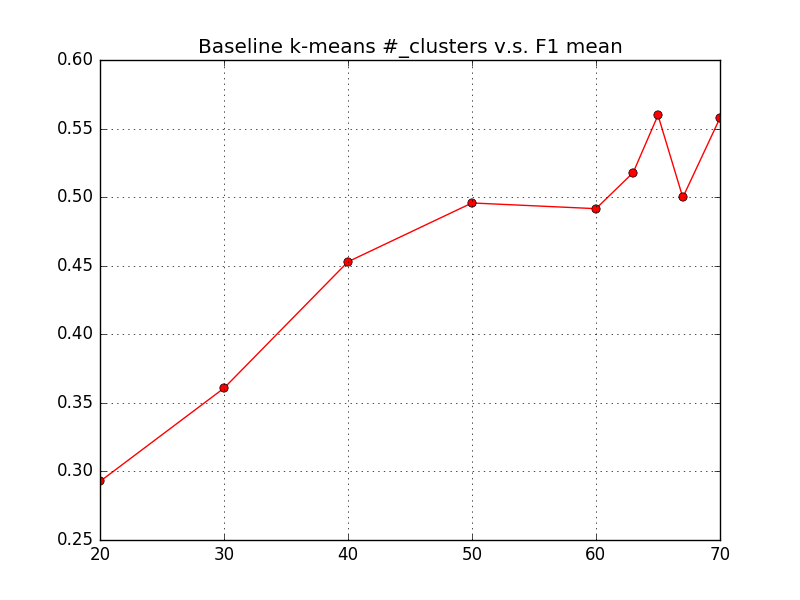
\includegraphics[scale=0.3]{Coarsefrom20to80.png}
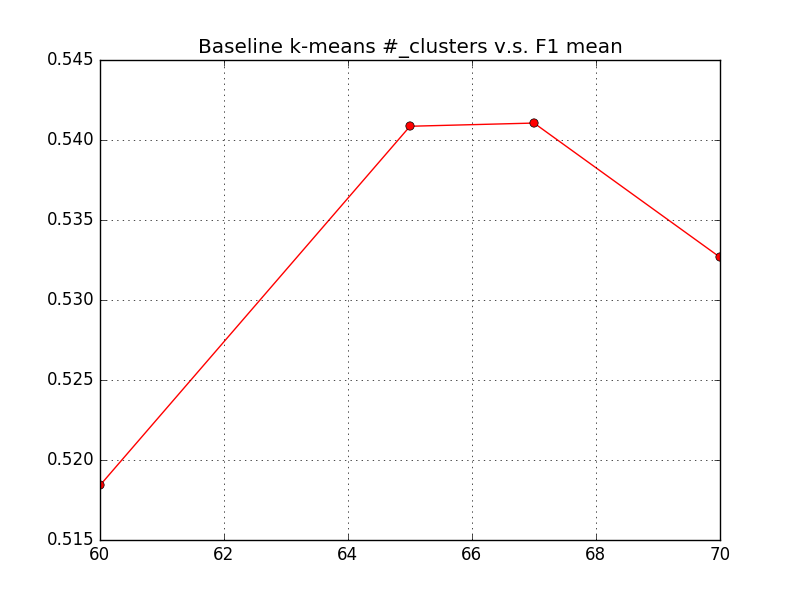
\includegraphics[scale=0.3]{finefrom60to70.png}
\end{center}

k=67. The mean is 0.541058776344, variance is 0.0007055614969. The best F1 out of 10 is 0.579381737382.\\
\subsection{k-means++ approach}
k=67. The mean is 0.551529967305, variance is 0.000512666340166. The best F1 out of 10 is 0.598781761183. \\

\subsection{Custom algorithm}
Keeping the kmeans++ initialization and kmeans iteration with cosine similarity scheme unchanged, my custom algorithm mainly replaces each term frequency in the term-document matrix with the tf-idf value.  
\[ tf-idf_{t,d} = tf_{t,d} \cdot \log \frac{N}{df_t}\]

This custom algorithm solves the problem in raw term frequency scheme where all terms are treated equal, however, it is not a proper way since some terms are less informative e.g. (stop words) or discriminative in contributing to the relevance score. For example, a collection of newswire is likely to have the term \textit{report} appears many times. We might want to attenuate the unwanted contribution that frequent terms make in scoring. Since we are discriminate documents in ranking, document frequency would be a better choice than the collection frequency (which counts multiple occurrences of a term.) Therefore it is a good choice to multiply the raw term frequency with the inverse document frequency, where taking log dampens the scaling down effect. I'm therefore trying to improve upon external metrics, e.g. F-measure, accuracy, NMI and purity, to improve the clustering quality and convergence rate to the underlining real class distribution. \\

k=67. The mean is 0.606431487906, variance is 0.000777387170029. The best F1 out of 10 is 0.658362769998.\\

\subsection{Analysis}
The custom algorithm (with tf-idf weighting, kmeans++ centroid initialization and cosine similarity measurement) achieves the best results. For the custom algorithm, the tf-idf weighting scheme worked out well and didn't increase much on computation cost. This improvement is desirable in that it emphasizes the informativeness of rare term while suppress the expressiveness of frequent terms. This follows the intuition that a term that occurs many times only within a small collection of documents must have high discriminating power to these documents v.s. others, which therefore better models the 1-versus-all classification problem or the clustering problem.\\

The baseline k-means performed worst but the performance gap is not large. This is due to the handling of empty clusters. Every time when a cluster got empty, we randomly pick a new point to the cluster. This is analogous to a random walk/reboot in the objective function and prevents iterations stuck into a relatively poor local minima. 
\subsection{Software implementation \& data preprocessing}
The software is developed under Python 2.7.10 with external scipy and numpy library for simple linear algebra operations and sparse data representation. It is includes modules: 1) load\_docVec (along with load\_customDocVec) where we construct a sparse matrix of term-document matrix; 2) random\_initializaiton (along with kMeansPlusPlus\_Initialization): where we select initial centroids in either way; 3) assignment: when we assign each document to one of the cluster; 4) update: when we update centroids based on the assignment result in this iteration; 4) main: this module chains the whole process together. \\

The major data structures include sparse matrix for term-document matrix M, dense matrix for centroids C, arrays for cluster labels, dict for document frequency, etc. Each document-centroid cosine similarity calculation is performed in a position-by-position case, where we read each normalized term frequency in M and each normalized term frequency in C, multiplies them together and sums over all terms to get a cosine similarity. \\

Included are Numpy and Scipy library. On the remote UNIX environment, numpy is installed but not scipy. PyCharm is used as the programming IDE. \\

My design strictly follows the kmeans/kmeans++ process. The modulars are highly in cohesion and low in coupling. Parameters can be tuned in an easy manner, by modifying the n\_cluster array to add more desired value of n\_cluster. Scipy and Numpy provides excellent support on scientific computation. The code is easier to understand than C++. Design in Python is efficient in implementation but the running time is relatively slower than C++/Java. There's by far no problem encountered by my system. \\

\subsection{Source code and test set results}
Please find the README.txt file for instructions on running the code. \\

Please also find the xinq-test-clusters.txt file as the final document clustering result on the test set. Thanks for your support!

\end{document}